\documentclass[tikz,border=5pt]{standalone}
\usepackage{pgfplots}
\pgfplotsset{compat=1.18}

\definecolor{corba}{HTML}{365FB3}
\definecolor{punt}{HTML}{B91C1C}
\definecolor{assimptota}{HTML}{6B7280}

\begin{document}
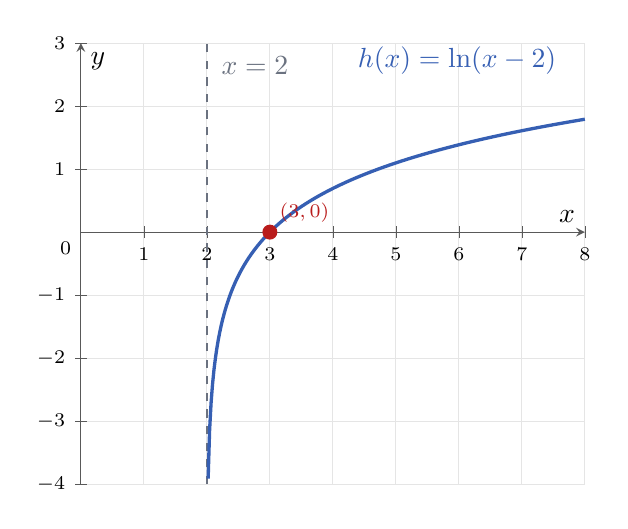
\begin{tikzpicture}
  \begin{axis}[
    width=8cm,
    height=5.6cm,
    scale only axis,
    axis equal image,
    axis lines=middle,
    grid=major,
    grid style={black!10},
    axis line style={black!65},
    tick style={black!65},
    tick label style={font=\scriptsize},
    xlabel={$x$},
    ylabel={$y$},
    xmin=0, xmax=8,
    ymin=-4, ymax=3,
    xtick={0,1,2,3,4,5,6,7,8},
    ytick={-4,-3,-2,-1,0,1,2,3},
    clip=false,
  ]
    \addplot[assimptota, dashed, thick]
      coordinates {(2,-4) (2,3)};
    \addplot[corba, very thick, domain=2.02:8, samples=260]
      {ln(x-2)};
    \addplot[only marks, mark=*, mark size=2.5pt, punt]
      coordinates {(3,0)};
    \node[anchor=north east, font=\scriptsize]
      at (axis cs:0,0) {$0$};
    \node[anchor=south west, text=punt, font=\scriptsize]
      at (axis cs:3,0) {$(3,0)$};
    \node[anchor=south west, text=assimptota]
      at (axis cs:2.08,2.35) {$x=2$};
    \node[anchor=south east, text=corba]
      at (axis cs:7.7,2.35) {$h(x)=\ln(x-2)$};
  \end{axis}
\end{tikzpicture}
\end{document}
